% !TeX spellcheck = en_US 
\chapter{Forensic audit and its computer support}


\komentar{na zacatek shrnout co vsechno obsahuje tato kapitola. asi tak takhle:}


This chapter strives to define and explain the meaning of the term "forensic audit" as well as other therms related to this field. We demonstrate typical roles and outline the process.
\komentar{az bude kapitola dopsana, zkontrolovat, zda toto odpovida} 

%\section{Matters of forensic audit}
%\komentar{nelibi se mi, pridat do jinych casti a zrusit}
%Forensic audit is a specialization within a field of accounting that examines and evaluates evidence concerning unproven statements for possible use as evidence in court. Forensic audit is usually used in case there is a suspicion in certain company there is a crime being committed. The background of the investigated case is rather diverse. A customer can be, for example, a CEO  who wants to examine the functioning of one of the sub-divisions of a controlling company. There can be a suspicion of some fraudulent activity or the need of forensic audit can be closely unspecified.

\section{Definition of forensic audit}\label{FA_definition}
The term "forensic" can be defined in multiple ways. According to merriam-webster dictionary \komentar{citace http://www.merriam-webster.com/dictionary/forensic} the definition is "relating to the use of scientific knowledge or methods in solving crimes". The term "audit" is explained in the same dictionary as "a complete and careful examination of the financial records of a business or person". \komentar{citace http://www.merriam-webster.com/dictionary/audit}

The essence of forensic audit is to discover and investigate fraudulent intentions and fraudulent behavior. 

A common mistake in the definition of forensic audit is to confuse it with financial audit. The aim of financial audit is to verify whether financial statements are fairly stated in accordance with accounting standards. Financial auditors search for material errors or other misstatements in the accountancy.

On the other hand the ultimate goal of forensic audit is to examine existing or gained suspicion and procure evidence concerning possible fraudulent behavior. Deceptive scenarios are discovered in the process of forensic audit and evidence together with a documentation that is usable for subsequent course of action is gathered. As a matter of principle forensic auditors are not expected to express their opinion on the guilt or innocence of suspects.


%\section{When to use forensic audit}
%\komentar{asi spis nez priklady popsat za jakych situaci...}
%\sediva{\blindtext}

%=============================ze stare BP========================================
\section{Types of investigation}

The range of types of situation that forensic auditor can be asked to investigate is really wide. Basically any kind of suspicion on potentially bad behavior can be an impulse for investigation. However, not all kinds of crimes are of our interest. For example violent crimes, cash theft, assault, robbery, rape, actual bodily harm and similar crimes are part of a detective work. Forensic auditors typically do not deal with such crimes. 

On the contrary, fraudulent crimes are those ideally fitting for forensic investigation. There are many different kinds of fraud that forensic auditors deal with. To provide an overview of the wide range, these frauds can be classified into following three groups: corruption, asset misappropriation and financial statement frauds. These frauds are the most frequently investigated scenarios.

\paragraph {Corruption}
Corruption can be characterized as a misuse of status. The motivation behind corruption is a desire to gain money, material possession or other advantages. By extension an involvement in a corruption relationship is a sign of moral and ethical failure of individuals. Several specific kinds of corruption are bribery, acceptance of a bribe, extortion, misuse of power, misuse of information or conflicts of interest. Research shows that corruption is involved in around one third of all frauds. \komentar{[citace Weaver]}

\paragraph{Bribery} is an unauthorized advantage in form of recipient's behavior alternation in exchange for money, goods or other forms of recompense. On contrary to bribery extortion occurs when money or some action is demanded in order to secure particular outcome. Conflict of interest and misuse of power or information can be categorized in one group. In such situations fraudsters use their power to achieve personal profit without regard to their position responsibility. Consequently their behavior negatively influences the company which is giving them their power. For example a manager of local division of a company choose his friend to be the paper supplier even though that his price is significantly much higher than the price of other paper suppliers.


\paragraph {Asset misappropriation}
is the theft or embezzlement of company assets by directors, other fiduciaries or employees. Is by far the most common economic crime experienced by organizations reporting any fraud, with 69\% of respondents suffering from it. \komentar{[citace http://www.pwc.com/gx/en/services/advisory/consulting/forensics/economic-crime-survey/economic-crimes/asset-misappropriation.html]} It happens when people who are entrusted to manage the assets of an organization steal from it. The stealing usually starts small and when perpetrators gain their confidence it becomes bigger. In consequence of this asset misappropriation can be a serious problem and can cause immense losses. 

The specific kinds are cash theft, inventory theft or using company assets for personal purpose. Special sort of asset misappropriation is fraudulent disbursement, i.e. for example fictional billing or raising an invoice that is not in compliance with the field of the supplier's enterprise. An interesting particularity is that asset misappropriation is far more likely to be committed by individuals than by a group of perpetrators.\komentar{citace http://www.theifp.org/research-grants/IFP-Whitepaper-5.pdf}


\paragraph {Financial statement fraud}
This kind of fraudulent activity is based on deliberate falsification of accounting records. It can include manipulation with expenses, manipulation of revenue figures, overstating assets or improper disclosure. This is regularly done to give the budgetary proclamations a specific inclination, for instance covering liabilities to enhance any examination of liquidity.

%====================================================================================
\section{Specializations in forensic audit}
The definition of forensic audit has already been stated in \ref{FA_definition}. However, there are several related specializations that can also be useful to know when dealing with this field.

\paragraph{Forensic Sciences} methodologically correctly apply broad spectrum of scientific disciplines in order to answer questions relevant to legal system. \komentar{[citace karin franke prednasky]} An aggregate of these sciences is sometimes also called simply forensics. Forensics is mainly used to deal with previously committed crimes or to prevent similar crimes from happening.


\begin{figure}[h]
	\begin{center} 
	%\missingfigure{Obrazek demonstrujici forenzni audit.}
	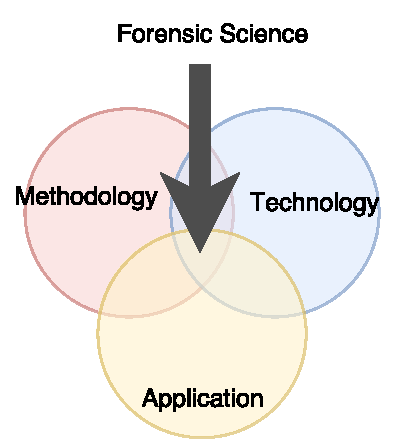
\includegraphics[width=0.4\textwidth]{img/forensic_science.pdf}
	\end{center}
	\caption{Forensic sciences}
\end{figure}


\paragraph{Computer (Digital) Forensics} is a discipline that studies digital evidence. It is used for recording, safeguarding, extraction and documentation of evidence from various kinds of hardware. Digital evidence sources are all kinds of digital equipment that is able to store usable pieces of information. These can be for instance computers, mobile devices, phones, deleted files, (surveillance) cameras, PDAs, copy machines etc..  Examples of digital forensics subbranches are mobile forensics, life-system forensics, file-system forensics, network forensics, multimedia forensics.  

\paragraph{Computational Forensics} is an research domain that uses the means of computational methods to study any kind of evidence. Computational forensics involves modeling, computer-based analysis, computer simulations etc.. This specialization uses methods such as machine learning, data mining, image processing, statistical pattern recognition, fuzzy logic or data visualization to discover any hidden forensic knowledge. 

\paragraph{} The subbranches of digital forensics as well as the specializations of computational forensics play their own part in the investigation of complex cases. They are used to provide intermediate results for the investigation by answering closely specified questions. Some of these methods can also be used indirectly as functionalities provided by a software that is used in the investigation.  

\komentar{

jine souvisejici oblasti forenzniho auditu
- specializace jako digital forensis etc.
vyuzitelne v ruznych pripadech na dilci vysetrovani
obnova dat - cesnet-man prednaska
(=> mohou se vyskytovat i dilci zakazky, kde se nezkouma komplexni situace ale napriklad jen obnovuji dulezita data, nebo analyzuji jednodussi pripady)


co nas zajima - situace, kde je vhodne uvazovat pocitacovou podporu
pocitacova podpora muze mit mnoho druhu-
vyuzivani konkretniho SW 
	analyticky, 
	statisticky, 
	podpora projektoveho managementu
	nastroje na sdileni informaci pri praci na projektu
vyuzivani nekterych obecnych principu 
	ctj. fuzzy logika,
		
	ctj data mining
		analyzovani zaznamu konverzaci,
		analyzovani vztahu mezi lidmi / chovani 
	strojove uceni?
	tyto principy mohou byt zakomponovane v nekterych konkretnich SW nastrojich vyse
vyuzivani konkretnich znalosti v pripade ziskavani dat z hw
	znalosti o fungovani operacnich systemu obecne
	znalosti o sitich
	konkretni znalosti o ukladani dat na disk
	tyto veci mohou slouzit jako nastroje na ziskani dukazu.

zdroje dat / dukazu
	zpracovatelne pomoci pocitace
		vypisy z uctu/ ucetnictvi, verejne databaze vlastnictvi, socialni site, elektronicka komunikace z dostupnych zdroju, znalosti / fakta o konktetnich osobach...
	nezpracovatelne pomoci pocitace, nebo vyuzivajici specificke principy sveho vlastniho oboru
		tady myslim sbirani otisku prstu a podobne oblasti, ktere resi specialiste



}


%============================^ze stare BP^=======================================





\section{How to prepare for a forensic audit}
%\komentar{v hrubych rysech jak to probiha (to co uz mam sem patri), na zaklade toho, co jsem zjistila, FA funguje takto:...\\}

On the basis of what we have found the process of forensic audit works as follows. When it is decided that certain situation will be investigated in forensic audit it is important to prevent all investigated individuals to access all related documents and electronic evidence. It is also recommended to limit their access to corporate information systems. 

Next step is to formulate properly the assignment. To define the extent and expectations on the outcome of forensic audit. To prevent a misunderstanding the assignment should be as specific and detailed as possible. It is best to choose the right audit company according to references and their experience with similar cases as the one we have specified.

When a client contacts an audit company with an assignment they usually schedule a meeting together, formulate sign and accept the assignment. The ordering party should be prepared to provide access to corresponding electronic and paper-like documentation as well as accept the fact that auditors are going to question employees and case-related person. On the other hand the audit company undertakes to refrain from sharing all the confidential information with third parties.A team of specialists that are convenient to the assignment is formed and the inspection is launched. 

In some cases the extent of the order is quite complex such as investigation of processes in one separate division of a company or investigation of complex corruption crimes. Nevertheless there may also be much easier cases where the audit firm is asked only to recover certain documents, or to examine particular piece of hardware. 

The following steps of precise methods of forensic audit are not definite. The ability to adapt in new situations is one of many essential capabilities for the team of forensic auditors. The variety of investigated cases is so vast that there is no universally valid and precise course of action in the same time. Therefore on this place we present only general methodology of forensic audit. Several selected methods of forensic audit will be described later in this document. \komentar{link na spravne misto!}

\section{General methodology of forensic audit}
In this section we present basic phases that are used while performing forensic audit. This process is most commonly divided into four stages: Accumulation, Examination, Analysis and Reporting. This basic methodology starts after the  selection of the audit company and after the specification of the assignment; at the same time when the real work of forensic auditors begins.

\begin{figure}[h]
	\begin{center} 
	%\missingfigure{Obrazek demonstrujici forenzni audit.}
	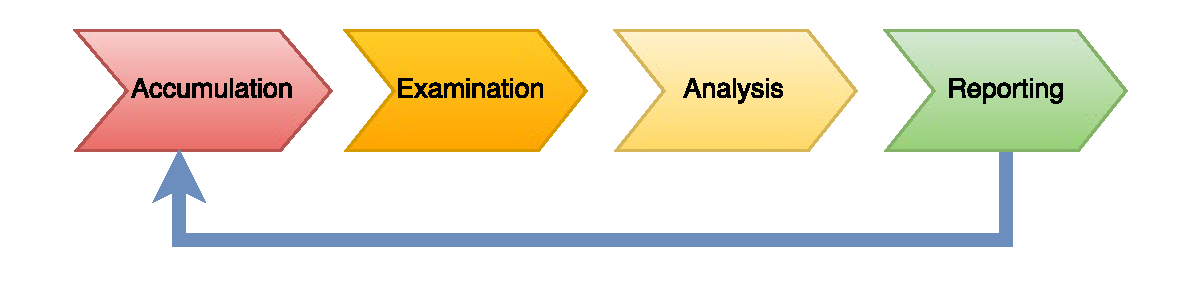
\includegraphics[width=1.0\textwidth]{img/general_methodology.pdf}
	\end{center}
	\caption{General methodology of forensic audit}
\end{figure}

%vvvvvvvvvvvvvvvvvvvvvvvvvvvvvvvvvvvvvvvvvvvvvvvvvvvvvvvvvvvvvv
\paragraph{Accumulation:} 
The main purpose of this stage is to acquire as much usable data as possible. It means recognize possible sources of data and provide backup record. All the sources of data and information, including necessary cross examination and other sources of evidence, should be utilized in this phase. All the information from the conceivable sources of pertinent information should be gained.

\paragraph{Examination:}
Examinations include forensically preparing all the gathered data. This can be done using a blend of computerized and manual systems to survey and concentrate specifically compelling information. 

\paragraph{Analysis:}
The following period of the procedure is to investigate the consequences of the examination, using legitimately reasonable routines and systems. The aim is to infer helpful data that addresses the inquiries that were the impulse for performing the accumulation and examination. \komentar{grrrrrr...}


\paragraph{Reporting:}
The last stage is reporting the consequences of the investigation, which may include depicting the activities utilized, clarifying how devices and methods were chosen, figuring out what different activities should be performed and giving proposals to change to approaches, rules, techniques, apparatuses, and different parts of the measurable procedure. 


%^^^^^^^^^^^^^^^^^^^^^^^^^^^^^^^^^^^^^^^^^^^^^^^^^^^^^^^^^^^^^^
%\sediva{\blindtext}





%===================================================================================
\section{Use case diagram of forensic audit in general}

As we see it there are three basic roles in forensic audit. A customer who wants a particular case to be investigated. The action of the customer is to assign the order to a audit company. A representative of the company i.e., for example, forensic auditor takes over the order and starts the investigation. The operations requiring specialized skills can be delegated to an expert from the proper field. Forensic auditors together with specialists then investigate the case and search for the evidence. In the end of the investigation the auditor reports the conclusion to the customer. 

\begin{figure}[h]
	\begin{center} 
	%\missingfigure{Velky obrazek vsech zainteresovanych stran - f.auditor, datovy analytik pro FA, zakaznik (zadavatel, materska spolecnost)}
	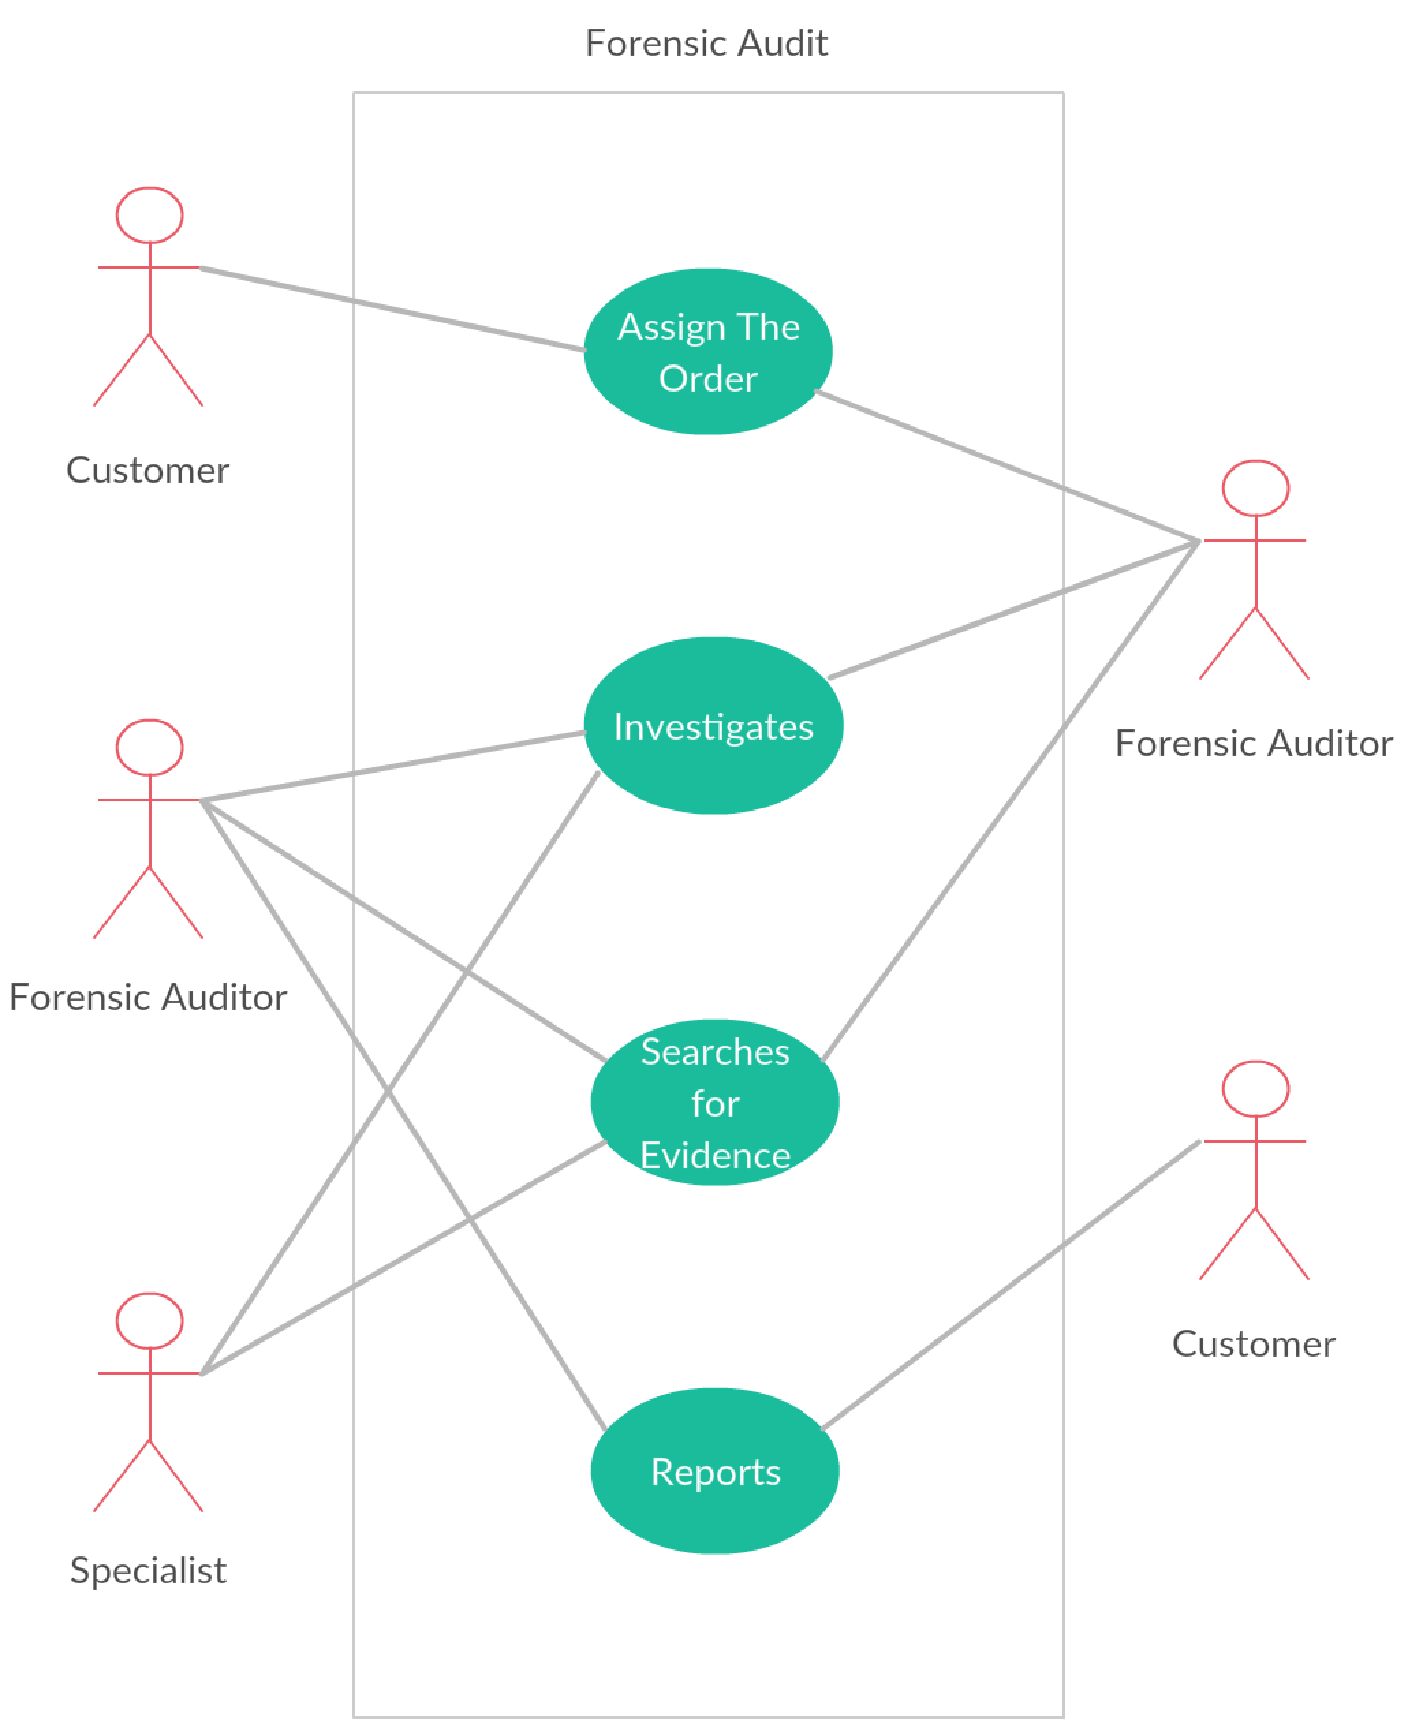
\includegraphics[width=0.8\textwidth]{img/usecase/use_case-FA_general2.pdf}
	\end{center}
	\caption{Use case diagram of forensic audit in general}
\end{figure}


\komentar{\section{co sem jeste zahrnout:}}
\komentar{
	VIZE: Rozdelit obecne druhy odhalovaneho chovani. Zahrnout vseobecne veskerou tresnout cinnost - nejspis podle zakona? Z techto oblasti vyelimimovat vsechny, pro ktere nema cenu uvazovat pocitacovou podporu (nasilne ciny, prepadeni, kradeze hmotneho majetku, pravni dokumenty? atd.). \\ Zbyle tak nejak rozdelit do skupin podle toho, jaky druh pocitacove podpory je obecne vyuzitelny. Pak se mozna pokusit k sobe priradit dany precin a metodu. Z metod nechci zminovat konkretni SW, ale spise obecne oblasti reseni - jak vyuzivame data mining, fuzzy logiku, strojove uceni (nebo alespon co to je a ze se take muze vyuzit), kvantitativne analyticky SW, forenzni toolkity na obnovu dat a podobne.
}

\komentar{
Priklady

·         Pan X, reditel ceske pobocky mezinarodni firmy\\

o   ma bratra, ktery mu dodava papir 500 Kc za balik.\\

·         Pani Y, ucetni spolecnosti\\

o   zauctuje falesnou fakturu na zalevani kvetin ve vysi 20 000 Kc (s vedomim pana Novaka)\\

·         Pan Z, spravce budovy\\

o    zamestna na parkovou upravu pred spolecnosti firmu, ktera mu stavi rodinny dum\\

Typy problemu\\

·         Predrazene dodavky\\

·         Fiktivni faktury\\

·         Nesoulad podnikani dodavatele a faktury\\

·         Paralelni spoluprace\\
}
%\dotaz{Z predchozi vize chci prejit v dalsi kapitole zpet k obecne metodologii a diagramu z ARISu. Nevim, jak na to plynule navazat aby to davalo celkove hlavu a patu. Snad me jeste neco napadne.}




